\chapter{Introduction}
\label{sec:intro}

The societal and economic impacts of climate change are expected to be some of the greatest stressors limiting a high quality of life in the coming century. Over 72\% of Americans view climate change as a moderate, serious, or imminent threat to the United States \cite{caspani}. The cost of limiting global temperature rise to 2\si{\celsius}, and assembling defenses against adverse consequences in the case that we fail, will be high. 

This introduction is written several weeks into the \gls{covid} pandemic quarantines that have so disrupted life in the United States and the world \cite{newsom,italy,india}. Already, many editorial columns of news outlets both international and local are comparing the scale of the present disruption to future catastrophes related to climate change \cite{wallace_wells,wyns,rosebrugh}. 

For instance, the shifting weather patterns induced by global warming are enabling new disease propagation paths, a public health crisis that has recently become particularly recognizable. The extreme weather events, extended dry/rainy seasons, and shifting crop pest populations linked to climate change will threaten the safety and livelihood of millions of people \cite{ahmed, smith_disasters}. When adjusted to January 2019 dollars, the total cost of extreme weather disasters in 2017 in the United States alone was \$312.7 billion, which is larger than the projected sum of all individual taxpayer rebates associated with the \gls{cares} Act \cite{smith_disasters,watson}. And in the absence of concrete climate change action, the World Bank Group projects that over 140 million people in Sub-Saharan Africa, South Asia, and Latin America will be displaced by changing water resources and crop productivity in areas affected by storms and rising sea levels \cite{wbg}. The ability to quarantine for extended periods of time is highlighting racial and wealth inequalities that will likely be reinforced and amplified by mass migration and other climate change stressors \cite{howell}.

At the forefront of the comparison between \gls{covid} and climate change is the realization that the human race lives within, and not apart from, a natural world that is at times unpredictable and difficult to control. And just as human travel has allowed a single-origin virus to affect almost every country on Earth \cite{who}, our shared atmosphere makes climate change a global phenomenon that can only be addressed through a collaborative effort. 

The purpose in making this comparison is not to prelude an otherwise impersonal and objective scientific work with a ``doom and gloom'' vision of the future. Neither is the purpose to imply that the technologies discussed in this dissertation are a silver bullet for these complex challenges facing humanity. Rather, the intention is to show that humanity is capable of making dramatic shifts in behavior of the kind needed to address climate change. 

Entire industries and many aspects of our daily lives must transition to low-carbon energy sources. Technological innovation in the energy space can be compatible with meeting our environmental goals. In a close second to the transportation sector, electricity production accounts for approximately 28\% of the total greenhouse gas emissions in the United States \cite{epa}. The vast majority of these emissions originate from the combustion of fossil fuels such as coal and natural gas. Nuclear fission power, which composes approximately 20\% of the electricity consumed in the United States, has life cycle greenhouse gas emissions comparable to wind and solar power \cite{ipcc} with a smaller land footprint \cite{strata}, higher capacity factor \cite{eia}, and lower worker and civilian mortality rates \cite{power_mortality} \hspace{0.02cm}\footnote{Most fatalities associated with wind and solar power manifest during equipment transport and as falls during maintenance activities \cite{wind_mortality,solar_mortality}.}.

Despite these favorable characteristics, public approval of nuclear power sits at 43\% in the United States\mdash just slightly above coal at 41\% and far below solar and wind power at 89\% and 83\%, respectively \cite{energy_approval}. Nuclear fission power is a mature technology that provides essential base load power that can complement daily and seasonal peaking of renewables; many projections of energy portfolios in carbon-limited scenarios include fission power as an important contributor to deep decarbonization of the electricity sector in tandem with energy diversification objectives \cite{mit_ne,iea_ne}. However, deploying nuclear power on the scale needed to evade the worst consequences of climate change requires addressing the societal, political, and economic issues currently limiting the technology's public approval.

In 2000, the United States \gls{doe} initiated the \gls{gif}, a collective of countries committed to the joint development of the next generation of fission reactors. After two years of deliberation, the Forum selected six reactor technologies believed to most effectively meet the future missions of nuclear energy with improved safety, economic feasibility, fuel cycle sustainability, and proliferation resistance relative to current commercial concepts. These six concepts include a \gls{vhtr}, a \gls{msr}, a \gls{scwr}, a \gls{gfr}, a \gls{sfr}, and a \gls{lfr}. The diversity in coolants, operating pressures and temperatures, and fuel cycles imparts unique advantages to each concept that make each design best suited to particular electricity markets, resource constraints, and energy missions.

This research develops and applies numerical models to \gls{th} analysis of \glspl{pbr}, a form of \gls{vhtr}. The \gls{vhtr} concept combines a gas or molten salt coolant with a graphite-moderated core to achieve very high temperature operation. Outlet temperatures are typically in the vicinity of 1000\si{\celsius}, high enough for process heat applications such as hydrogen production, coal gasification, and desalination. The \gls{vhtr} is expected to contribute significantly to deep decarbonization of the industrial sector, which accounts for 22\% of total greenhouse gas emissions in the United States \cite{epa}. 

Two different \gls{vhtr} fuel designs have been typically proposed. The first is a prismatic, fixed block-type fuel element such as that shown in Fig.\ \ref{fig:fuela}. Hundreds of these blocks are stacked in the shape of a cylindrical bed to form the reactor core. The second is a spherical fuel element, or ``pebble,'' such as those shown undergoing inspection in Fig.\ \ref{fig:fuelb}. Hundreds of thousands of these pebbles are heaped in an unordered manner within a cylindrical vessel to form the reactor core. This latter design, which is the focus of this research, is more specifically referred to as a \gls{pbr}.

\begin{figure}[!h]
\centering
\begin{subfigure}{.485\textwidth}
  \centering
  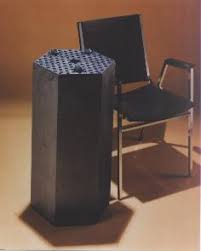
\includegraphics[height=0.6\linewidth]{figs/prismatic.jpeg}
  \caption{Prismatic fuel element block}
  \label{fig:fuela}
\end{subfigure}
\begin{subfigure}{.485\textwidth}
  \centering
  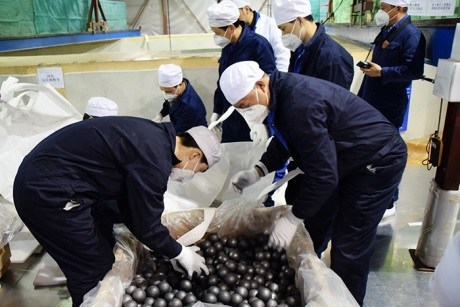
\includegraphics[height=0.6\linewidth]{figs/htr_inspection.jpg}
  \caption{Pebble fuel under inspection}
  \label{fig:fuelb}
\end{subfigure}
\caption{Photos of (a) a prismatic fuel element with a chair for scale \cite{ge_fuel} and (b) pebble fuel elements under inspection \cite{htrpm_fuel}.}
\label{fig:fuel}
\end{figure}

Section \ref{sec:pbr_concept} introduces the salient aspects of the \gls{pbr} design that distinguish the concept from both current commercial designs and the other concepts proposed by the \gls{gif}. The combination of a robust fuel form, passive heat removal systems, and high thermal efficiency make the \gls{pbr} a potentially significant contributor to meeting greenhouse gas emissions targets with improved safety and economic feasibility relative to current commercial reactors.

A notable characteristic of all \glspl{pbr} is a large separation of length scales between the fissile regions in each pebble and the full core. Section \ref{sec:ph_motivation} motivates the role of \gls{th} modeling in reactor analysis with emphasis on the constraints imposed by this large scale separation. Multiscale analysis, a branch of numerical modeling based on decomposing complex systems into separable models for each of the most important characteristic scales, is introduced as one means for achieving fast, design-capable, predictions of \gls{pbr} thermal and flow physics.

After having highlighted important \gls{pbr} \gls{th} phenomena in Section \ref{sec:ph_motivation}, Section \ref{sec:history} sketches a history of the \glspl{pbr} built and operated around the world. Attention is placed on the operational experiences that exemplify the importance of having accurate \gls{th} models of \glspl{pbr} with respect to predicting the thermal and safety design criteria introduced in Section \ref{sec:ph_motivation}. Finally, Section \ref{sec:outline} motivates the methods development and application performed in this dissertation and provides an outline for the remainder of this work.

% TODO: some other kind of big wrap-up here about an opportune moment, etc. Could also be at the very end.

% education plays an important role

% inherent and passive safety issues
% smaller reactors

% not just about climate change, but about helping bring power to all of the world - reference for energy consumption tied to quality of life?

%This is an opportune moment when our shared responsibility for addressing climate change is quite clear.  

%We are accountable to ourselves for delays to action and have a new appreciation for the role of science-based decision making.


%The main driver of climate change is the combustion of fossil fuels, and as such is closely tied to air pollution. The \gls{who} estimates that a million lives could be saved each year worldwide solely due to reductions in air pollution if the goals of the Paris Agreement are met \cite{who_pollution}.

% introduce the use of different coolants - gases and salts, but emphasize that the methods developed in this dissertation apply to both

\section{The Pebble Bed Reactor}
\label{sec:pbr_concept}

The defining characteristic of \glspl{pbr} is the use of spherical fuel elements, or ``pebbles.'' Following an early exploratory phase in the 1960s \cite{claxton,hecker}, the multitude of proposed fuel designs have converged to the coated particle form shown in Fig.\ \ref{fig:pbr_fuel}. A typical fuel pebble is 6 \si{\centi\meter} in diameter, slightly smaller than a tennis ball. A central core contains tens of thousands of \glspl{cfp} mixed in graphite. This ``fuel-matrix'' region is protected from erosion by a 0.5 \si{\centi\meter} thick graphite shell on the pebble surface. Each \gls{cfp} is approximately 1 \si{\milli\meter} in diameter and consists of a central kernel of fissile material, typically \gls{uo2} or uranium oxycarbide, surrounded by several layers of structural reinforcement materials \cite{demkowicz, powers}.

\begin{figure}[!h]
\centering
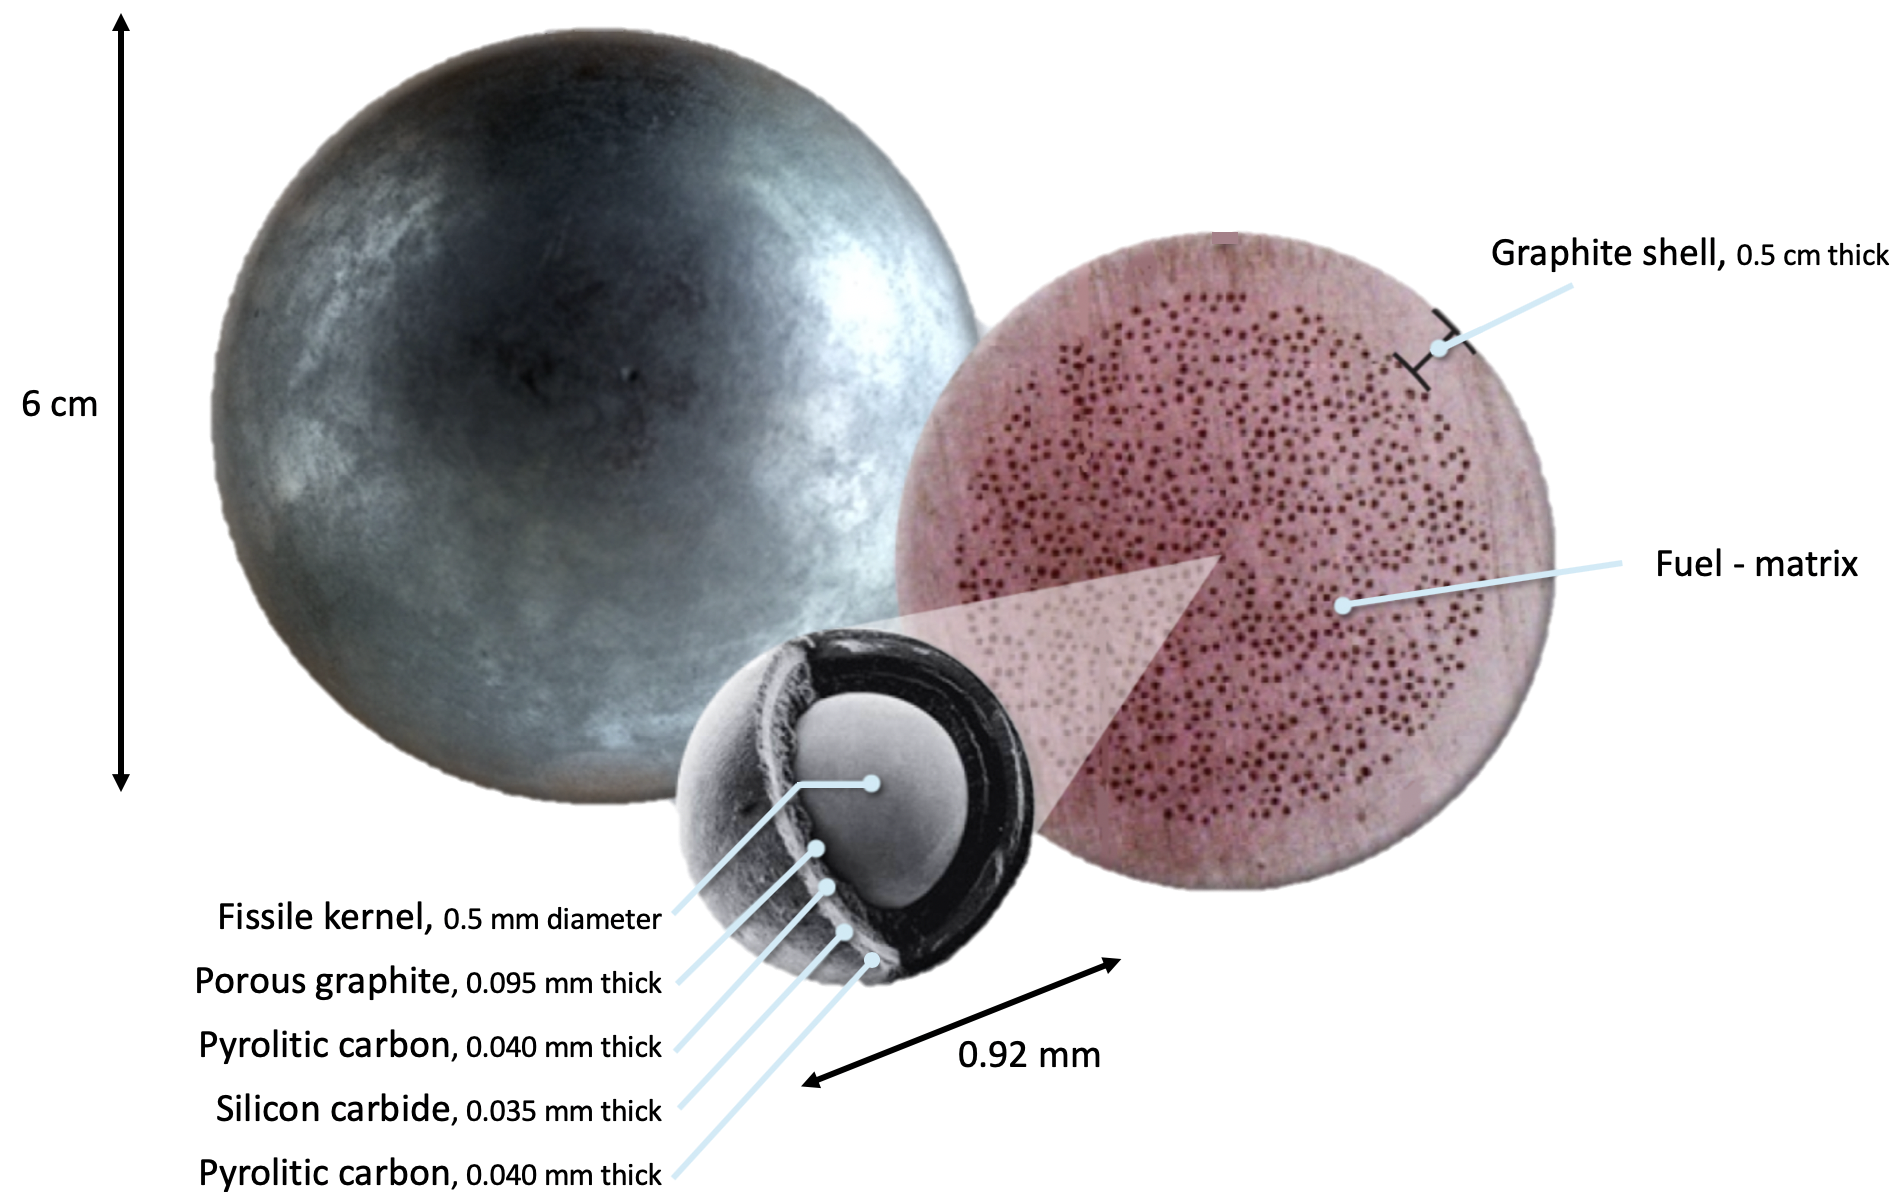
\includegraphics[width=0.6\linewidth]{figs/pbr_fuel.png}
\caption{Typical \gls{pbr} fuel pebble shown from the outside and along a cut-through, with an enlarged \gls{cfp} consisting of five layers (adapted from \cite{x_energy_pebble}).}
\label{fig:pbr_fuel}
\end{figure}

The first of these layers surrounding the kernel is a porous graphite ``buffer'' layer that retains gaseous fission products and accommodates kernel swelling. The \gls{cfp} shown in Fig.\ \ref{fig:pbr_fuel} is more specifically referred to as a \gls{triso} particle due to the use of three additional layers around the buffer\mdash a \gls{sic} layer sandwiched between two \gls{pyc} layers\hspace{0.02cm}\footnote{Pyrolitic carbon has a structure similar to graphite, and is formed by depositing gaseous hydrocarbon compounds onto a substrate.}. The \gls{sic} layer is the main pressure vessel for the particle and a diffusion barrier for gaseous and metallic fission products, while the \gls{pyc} layers protect the kernel from damage during the \gls{sic} deposition process and the \gls{sic} from damage during mixing of the particles with the graphite matrix. The robust high-temperature performance of the \gls{triso} particle allows long-term operation at fuel temperatures up to 1250\si{\celsius} and short-term transient operation at fuel temperatures up to 1600\si{\celsius} \cite{nabielek,demkowicz}.

Alternative \gls{cfp} designs exist with different layer structures from the \gls{triso} design show in Fig.\ \ref{fig:pbr_fuel}, though the predominance of the \gls{triso} particle design has led to the generic term ``\gls{cfp}'' being interchanged with the more specific ``\gls{triso} particle'' term in the literature. For generality, ``\gls{cfp}'' is used throughout this dissertation when describing methods that apply equally to other particle designs.

A typical \gls{pbr} core consists of hundreds of thousands of pebbles arranged in a random heap within a cylindrical enclosure formed by loosely-stacked graphite blocks. Fig.\ \ref{fig:corea} shows a plan view of the \gls{htr10} core before loading pebbles and Fig.\ \ref{fig:coreb} shows a photo of the \gls{thtr} bed with control rods inserted directly into the pebble region. Most \glspl{pbr} operate in an online refueling mode, where pebbles are continuously added to the bed, cycled through over the course of several months, and removed at the opposite end. Most reactors operate in a multi-pass scheme where each pebble is re-inserted into the bed two to ten times until the desired burnup has been achieved.

A coolant flows in the interstices between pebbles to remove fission heat. This energy is transported to a power conversion system that generates electricity with a Rankine or Brayton cycle and/or process heat for industrial applications. Upon entering the reactor core, the coolant typically first encounters an open plenum before flowing into the pebble region. In gas-cooled systems, this plenum is present on the top of the bed; pebbles are typically inserted into the core by a free-fall of several meters before hitting the upper surface of the bed. Conversely, the buoyant pebbles used in salt-cooled designs locates the plenum below the bed. In both gas- and salt-cooled designs, the coolant then exits the bed through thousands of ``suction holes'' machined in the reflector blocks that connect the core to the hot legs. The entrance to this outlet plenum geometry is visible in Fig.\ \ref{fig:corea} as the thousands of circular channels machined on the lower angled faces of the bed.

\begin{figure}[!h]
\centering
\begin{subfigure}{.485\textwidth}
  \centering
  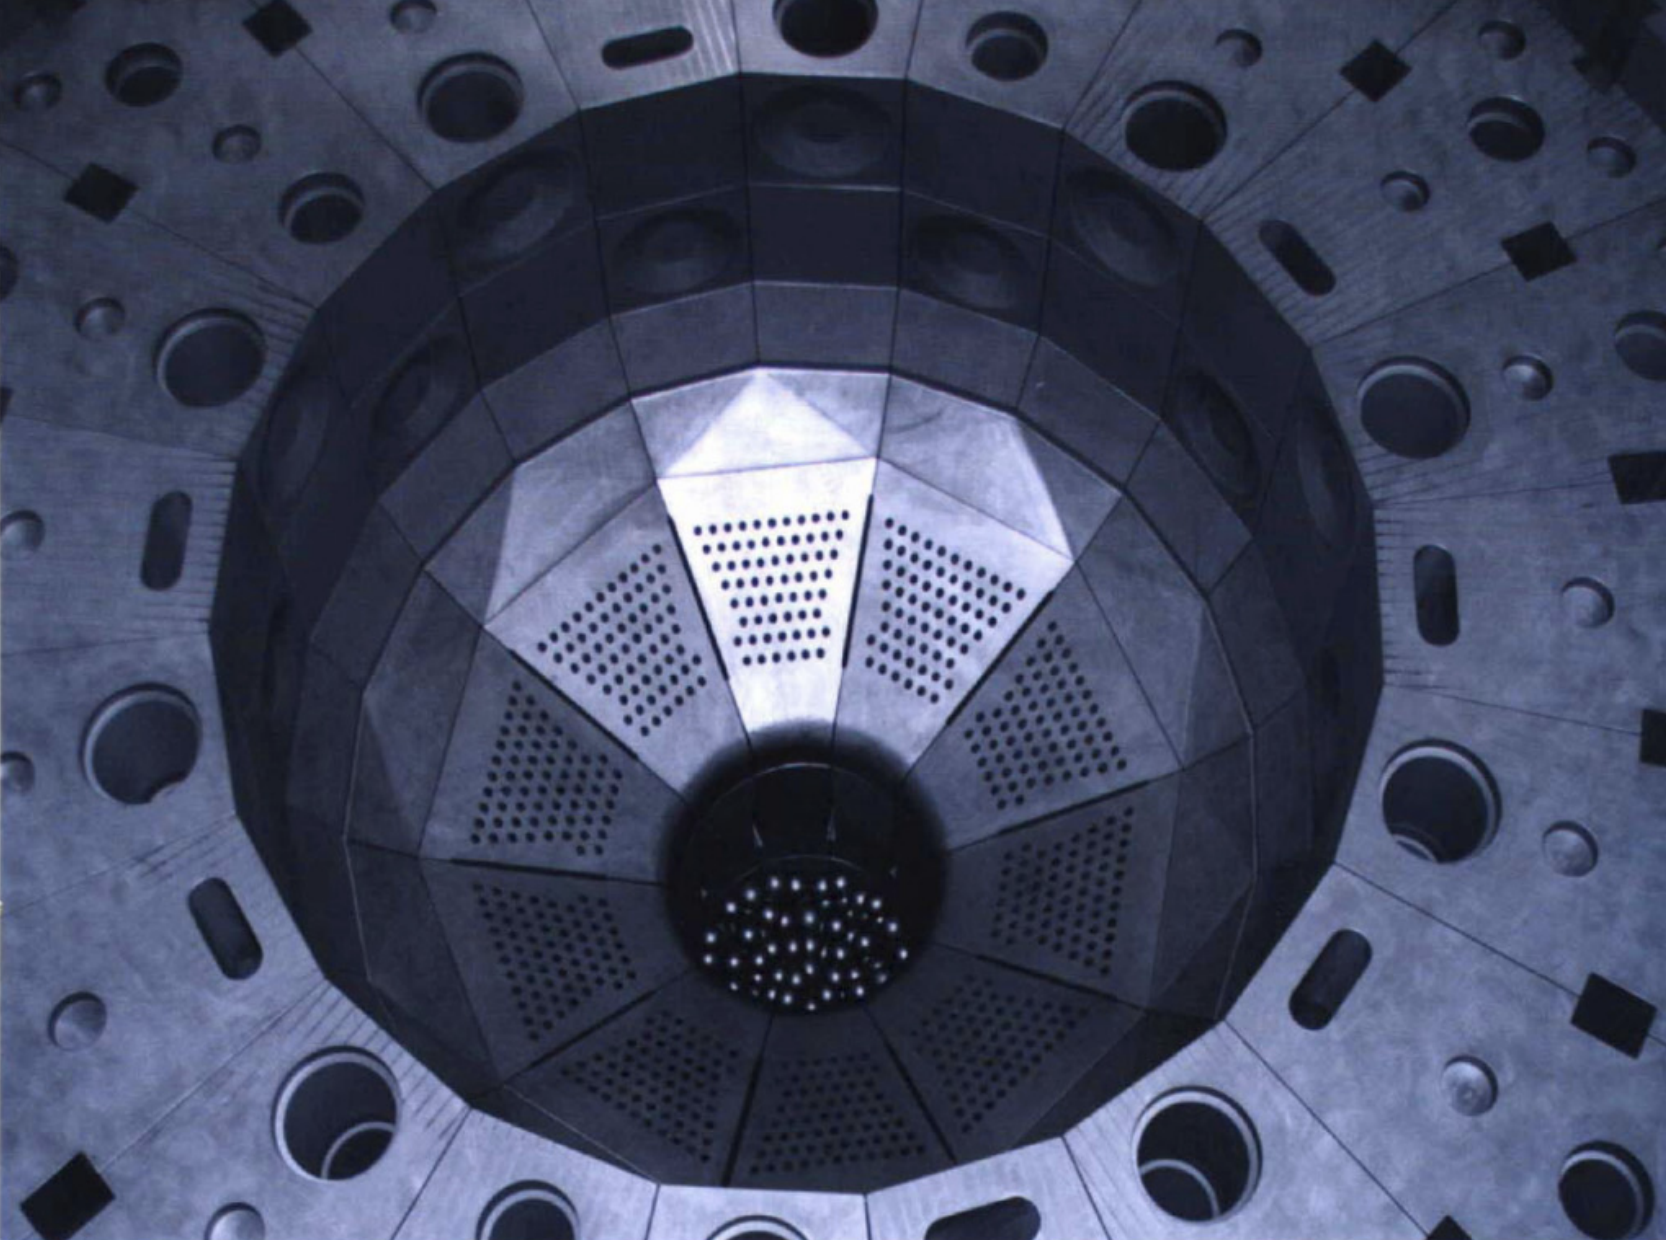
\includegraphics[height=0.5\linewidth]{figs/htr10.png}
  \caption{Plan view of mostly empty HTR-10 core}
  \label{fig:corea}
\end{subfigure}
\begin{subfigure}{.485\textwidth}
  \centering
  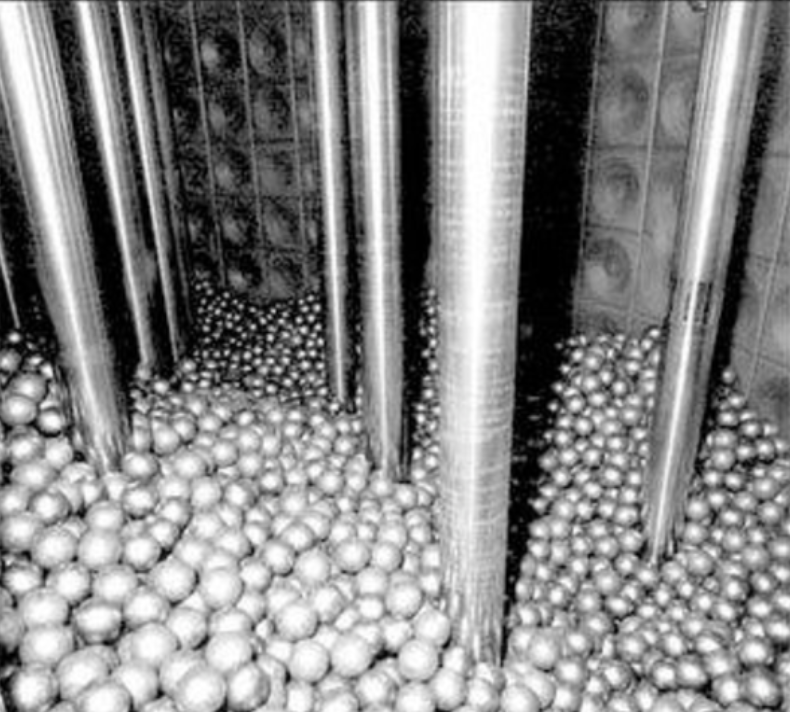
\includegraphics[height=0.5\linewidth]{figs/thtr_core.png}
  \caption{Filled core region of the THTR}
  \label{fig:coreb}
\end{subfigure}
\caption{Photos of the (a) \gls{htr10} core before loading of pebbles \cite{HTGRLessonsLearned} and (b) the \gls{thtr} core with control rods inserted directly into the pebble bed \cite{thtr_core}.}
\label{fig:core}
\end{figure}

In addition to the flow paths through the pebble bed, a number of additional ``bypass'' routes divert coolant from the fuel. In the \gls{htr10} shown in Fig.\ \ref{fig:corea} for example, the outer reflector consists of circular and oblong flow channels that accommodate control rods, backup control systems in the form of loose absorber pebbles, and reflector cooling channels. Coolant may also flow through \si{\milli\meter}-size gaps that form between the reflector blocks due to temperature- and irradiation-induced deformation. Within the bed, pebble ordering near walls also introduces an in-core bypass due to a reduced flow resistance. Both the \gls{htr10} in Fig.\ \ref{fig:corea} and the \gls{thtr} in Fig.\ \ref{fig:coreb} incorporate ``subwoofer''-shaped dimples to disrupt this near-wall pebble alignment.

\glspl{pbr} have a number of economic and safety advantages relative to other reactor concepts. The robust and resilient coated particle fuel form allows long-term operation at high temperature. With proper coolant and structural material selection, \glspl{pbr} may operate at significantly higher coolant temperatures than other reactors. For example, the coolant outlet temperature of the \gls{thtr} was 750\si{\celsius}; about 325\si{\celsius} higher than that of the \glspl{lwr} comprising approximately 96\% of today's commercial reactors \cite{reactor_count}. High temperature operation improves the thermal efficiency of electricity production and expands nuclear power to industrial process heat applications, which represent almost 10\% of total carbon emissions worldwide \cite{friedmann}.

The use of an on-line refueling scheme enables operation with low excess reactivity, which reduces requirements of burnable absorber and control systems and attendant burnup penalties. Provided component accessibility and dose rates permit on-line maintenance, multi-week service and refueling shutdowns may be significantly reduced, increasing reliability and net kWh produced. For multi-pass schemes in particular, frequent opportunities to observe pebble integrity may reduce the coolant source term and lower off-site dose rates. A more fine-grained control of individual pebble burnup may also improve overall fuel utilization relative to fixed-fuel reactors.

Most \gls{pbr} designs use a gaseous coolant such as helium or a liquid coolant with high melting and boiling points such as \gls{flibe} salt. For designs that also incorporate Brayton power conversion cycles, the use of non-water coolants may eliminate the need to site power plants near large natural or engineered bodies of water and support related environmental impact programs such as stocking programs that replenish fish impinged by water intake pipes \cite{exelon_fish}. The use of single phase coolants also eliminates many of the operational difficulties associated with two phase liquid-vapor flow such as density-wave oscillations.

The large quantities of high heat capacity graphite in \gls{pbr} cores greatly extends the time scale of thermal transients. Hours or even days may pass before peak temperatures are reached following certain events such as a \gls{loca} \cite{htrpm,tyobeka}. Slowly-evolving transients that characterize some non-water reactor types mean accidents evolve slowly and therefore provide additional time for human operator response and activities such as equipment repair or substitution should equipment be damaged in an accident.

As with any system designed based on multiple constraints and trade-offs, there are a number of complexities and disadvantages associated with the \gls{pbr} concept. The fuel pebble shown in Fig.\ \ref{fig:pbr_fuel} is approximately 98.2\% graphite by volume, with the remaining 1.8\% occupied by the fissile kernel and \gls{sic}. While large quantities of graphite extend thermal transients, \glspl{pbr} are generally restricted to power densities two to three orders of magnitude lower than other designs such as \glspl{lwr} and \glspl{sfr}. The relatively large reactor vessels of \glspl{pbr} complicate rail transport, contribute significantly to structural material costs, and increase waste volumes.

However, many \gls{pbr} designs refashion power density restrictions to their advantage by employing passive decay heat removal mechanisms that would otherwise be incapable of transporting orders of magnitude higher volumetric heat generation from the core. Power densities are typically low enough that radiation and conduction between touching pebbles, in combination with an ex-vessel cooling system, is sufficient to remove decay heat in a depressurized \gls{lofc} accident by natural convection cooling. However, the high surface areas required to achieve the needed heat removal rate by the ex-vessel cooling system often impose a leakage penalty.

The constant abrasion and frictional wear as pebbles move through the bed may generate significant quantities of graphite dust \cite{hecker,moormann}. In gas-cooled designs, solid fission products tend to accumulate in this dust and transport about the primary system in an unpredictable manner, complicating analysis of depressurization events and decommissioning activities due to the mobile and inhalable source term. Instruments and fittings may also not perform as intended in the presence of dust layers. While lubrication in salt coolants may alleviate many operational issues associated with dust generation, additional engineering systems are required to manage this unique solid-solid erosion source term.

In some early fuel designs, the fuel-matrix region was formed as a loose mixture of graphite ``flour'' with \glspl{cfp} to simplify fuel recycling \cite{claxton, hecker}. Reprocessing technologies for graphite-coated \glspl{cfp} today have not progressed beyond the laboratory scale, complicating the ability to close the fuel cycle \cite{moses} but likely reducing the proliferation potential of the \gls{pbr} open fuel cycle.

The high thermal efficiency, passive safety, and high-temperature resilient pebble fuel form of \glspl{pbr} offers great potential to decarbonize the electric and industrial heat sectors. Natural convection decay heat removal and a high thermal inertia contribute to slower transient progression even in the absence of human intervention. However, the low power density, lack of a thriving fuel supply chain or commercial-scale reprocessing technology, and engineering challenges such as dust generation require consideration of these trade-offs in determining the particular markets and missions best suited to commercial deployment. Continued \gls{rd} in the \gls{pbr} space will improve the engineering design of these systems to further enhance the viability of this technology.

% something about small modular reactors?

\subsection{Thermal-Hydraulic Modeling and Simulation}
\label{sec:ph_motivation}

The objective of \gls{th} \gls{ms} of \glspl{pbr} is to vet designs against thermal, mechanical, and radiation limits bounding safe, reliable, and economical operating spaces. Fast-turnaround analysis tools enable more rapid design iterations and scoping studies at significantly lower cost than the long lead-time experimental programs typical of nuclear engineering. As a non-nuclear example, Boeing transitioned from mockup-based experimental programs to heavy reliance on \gls{ms} for the engineering design of the Boeing 777 aircraft. The shift in emphasis from physical experiments to numerical experiments reduced the number of engineering change requests by 90\% and the cycle time for incorporation of a design change by 50\% \cite{boeing}.

For \gls{ms} to be a valuable design tool for reactor development, numerical models must be able to characterize the proximity of the reactor state to the thermal, mechanical, and radiation limits bounding the desired operating space. These limits are expressed in terms of a number of physical metrics that correlate with component damage, worker and civilian dose rates, and degraded economic performance. The ability to effectively cool the fuel is often used as a secondary metric to indicate fuel/core damage and radiation release to the coolant. For the \gls{th} models that are the topic of this dissertation, \gls{ms} tools must be able to accurately predict

\begin{itemize}
\item Maximum coolant outlet temperature, or the highest temperature of structural components that must be maintained below material damage thresholds. The maximum coolant temperature is also correlated to chemical reaction rates such as corrosion.
\item Minimum coolant temperature and freezing-related geometry changes that may reduce fuel cooling.
\item Gradients in the coolant outlet temperature, which result in fluid mixing and cyclic thermal fatigue to structural materials.
\item Maximum fuel temperature, which is correlated to various fuel failure modes that may result in damage and radiation release. Even in the absence of observable damage, the maximum fuel temperature correlates with fission product diffusion coefficients and the coolant source term.
\item Core pressure drop, which is indicative of the pumping power required to cool the core and the feasibility of natural convection decay heat removal in pump loss transients.
\item Fluid-structure interaction and vibration-induced failure modes.
\item Radiation damage and the resulting material dimensional changes and degradation.
\item Radiation activation of the coolant and structural materials.
\item Large-scale structure failure such as pipe breaks.
% add reflector temperature?
\end{itemize}

The physics correlated by these metrics consist of a mixture of core-level phenomena, such as feasibility of natural circulation, and particle-level phenomena, such as fuel particle layer integrity. Recall that a typical \gls{pbr} core consists of a roughly 10 \si{\meter} tall cylindrical vessel containing hundreds of thousands of \si{\centi\meter}-size fuel pebbles, each of which consists of thousands of \si{\milli\meter}-size \glspl{cfp}. The localization of the heat source to small fissile kernels, the thermal resistance of the \gls{cfp} layers surrounding the fissile kernels, and the core-wide fission power distribution all contribute to significant variation in most \gls{th} phenomena of design interest to \glspl{pbr} over five orders in spatial magnitude. Accurate prediction of the thermal and flow metrics listed above requires model resolution of

\begin{itemize}
\item Heat conduction and material performance in \(5\times10^9\) fuel particles\hspace{0.02cm}\footnote{Assuming roughly \(5\times10^5\) pebbles and \(1\times10^4\) particles/pebble}; 
\item Intra-pebble heat conduction; inter-pebble conduction and radiation; and pebble-fluid convection and frictional resistance for \(5\times10^5\) pebbles; and
\item Large-scale interactions of the pebble-coolant system with spatially-dependent fission power, \glspl{bc}, and material properties; reactor control systems; and the \gls{bop} for power generation.
\end{itemize}

\gls{pbr} core analysis is further complicated by its stochastic geometry. Both the \gls{cfp} positions within each pebble and the pebble arrangement within the bed are stochastic. On-line refueling results in a continuous distribution of thermal properties and burnup that are also stochastic. Average packing distributions and granular flow properties are well-quantified for beds of spherical pebbles, while \gls{cfp} positions can usually be approximated with non-overlapping \gls{rsa} methods \cite{jodrey}. However, ensemble averaging is still required to characterize the effect of randomness on the \gls{th} parameters of interest.

\gls{th} models that fully resolve all \glspl{cfp}, pebbles, and the surrounding coolant require about \(10^{12}\) elements in the fluid phase to capture the complex fluid-solid interfaces and boundary layers \cite{wu2010} and about \(10^{15}\) elements in the solid phase to resolve the multiple thin layers on the thousands of \glspl{cfp} in the hundreds of thousands of pebbles \cite{novak_2019}. Furthermore, mesh generation near pebble contact points is often characterized by significant skew that degrades numerical convergence; methods to systematically improve mesh quality in these regions without distorting the porosity remain an open research question \cite{dixon,nijemeisland}.

Most \gls{pbr} beds are surrounded by a graphite block-type reflector that contains flow channels to accommodate control rods, absorber spheres, and coolant flow paths. Horizontal and vertical gaps with widths on the order of \(10^{-3}\) \si{\meter} form between the blocks as a function of irradiation and temperature \cite{guo_2018,liu_sas}. The engineered flow channels, in combination with these gaps, permit bypass flow paths that simultaneously cool the reflector and core externals while diverting coolant from the fuel. These reflector bypass flows therefore have important effects on thermal stresses, overall component lifetime, and uniformity of outlet temperatures, and must be considered in core \gls{th} analysis \cite{guo_2018,anderson}. However, coupling the reflector bypass flows to a bed \gls{th} model greatly increases the size of the simulation domain and requires judicious mesh generation for a geometry consisting of a mix of very thin gaps and comparatively large engineered channels.

Such ``high-resolution'' models, which fully resolve all geometric scales in the pebble bed and reflectors, are intractable for the fast-turnaround calculations needed for routine reactor design and analysis. The ``everyday'' computing resources available to regulatory agencies and the nuclear power industry are typically single-user, multi-core, workstations sized to perform tens to hundreds of design iterations per day \cite{nrc_nonlwr}. While high-resolution models are invaluable for benchmarking lower-resolution tools, generating closures, and exploring fine-scale phenomena, supercomputing resources currently limit these calculations to homogeneous pebble interiors in either a random heap of several hundred pebbles or a regular lattice with symmetry conditions\mdash far short of the hundreds of thousands of pebbles, and their heterogeneous interiors, constituting a \gls{pbr} core \cite{calis,zhang2016,baker_2010,alkhalaf,guardo,gunjal}.

Multiscale analysis is a branch of applied mathematics that is based on decomposing a complex system into a number of important temporal and/or spatial length scales, each described by different models, that are then aggregated together to obtain a representative physics solution over many orders of magnitude in time and/or space. Provided the models for each characteristic scale are sufficiently simple, the computational cost of a multiscale decomposition may be orders of magnitude lower than a fully-resolved model. 

This dissertation develops and applies multiscale models to \gls{th} analysis of single-phase \glspl{pbr}. These multidimensional models are of ``intermediate'' fidelity\mdash they are lower in resolution than the fully-resolved models described in the preceding paragraphs, but higher in resolution than the 1-D flow network models used for loop analysis or the pseudo 3-D subchannel methods used for primarily unidirectional flows. Before outlining the work performed in this dissertation in Section \ref{sec:outline}, Section \ref{sec:history} provides a brief history of \gls{pbr} \gls{rd} around the world with emphasis on operating experiences that highlight the importance of having accurate models of \gls{pbr} \gls{th}. 

\subsection{A Brief History in the Context of Thermal Analysis}
\label{sec:history}

This section traces a brief history of the design, development, and operation of \glspl{pbr} around the world to demonstrate the relevance of the methods developed in this dissertation to predicting complex and engineering-significant phenomena in \glspl{pbr}. For brevity, emphasis is placed on programs that resulted in construction and operation of a \gls{pbr} or that are currently engaged in doing so. The reader is referred to the literature for more comprehensive chronologies \cite{claxton,thomas}. And rather than attempt a complete technical description of each \gls{pbr} design, attention is focused on the operational experiences that call attention to the engineering significance of the thermal safety and reliability criteria introduced in Section \ref{sec:ph_motivation}. This section concludes with an in-exhaustive survey of several concepts under development in the United States and abroad to highlight the wide variety of systems that multiscale models must consider.

In the late 1950s, a group of 15 utility and power supply companies united as \gls{avr} GmbH with German government support to construct the first \gls{pbr}\mdash a 15 MWe, helium-cooled, reactor in J{\"u}lich, Germany \cite{hecker,oehme,nrc_avr,moormann}. The purpose of this project was to explore the \gls{pbr} concept and its technical feasibility for electricity and process heat applications. This reactor, referred to as the \gls{avr}, achieved first criticality in 1966 and operated for over 20 years, providing invaluable technical experience and demonstrating the feasibility of many aspects of the \gls{pbr} design such as fuel handling systems, \gls{bop} components, and gas purification processes. Many key safety aspects of \gls{pbr} designs were verified; a series of progressively evolving \gls{cfp} fuel forms exhibited excellent fission product retention at high temperatures, while \gls{lofc} experiments proved natural circulation to be capable of safely removing decay heat. The \gls{avr} also set the world record for highest sustained outlet temperature of a nuclear reactor\mdash990\si{\celsius}.

One of the more well-known experiments conducted in the \gls{avr} involved the measurement of bed temperatures during steady-state operation. Due to the difficulty of obtaining temperature readings within a moving, random heap of pebbles, 120 non-fissile instrumented pebbles were loaded into the bed, cycled through, and removed after a single pass. Fig.\ \ref{fig:avr_melt} shows a picture of one of these instrumented pebbles; a center plug contains a wire with a known melting temperature. With 20 different wire materials and two load locations, a very coarse temperature map was obtained. The majority of pebbles indicated temperatures up to 200\si{\celsius} higher than permitted in the reactor license \cite{sobes,moormann}. And, depending on location, between 7 and 31\% of the pebbles exceeded the maximum wire melting temperature of 1280\si{\celsius}; coarse estimates suggest these pebbles exceeded allowable temperatures by as much as 240 to 340 \si{\celsius}. Decades later, improved computational models and an improved understanding of \gls{pbr} \gls{th} suggests that a large contributor to these high temperatures in the \gls{avr} was neglecting bypass flow through control rod channels and gaps formed between the carbon insulation and the reactor shroud \cite{viljoen}, though it is likely that hot spot formation also played an important role \cite{moormann}.

\begin{figure}[!h]
\centering

\includegraphics[width=0.4\linewidth]{figs/avr_melt_wire.png}
\caption{Non-fissile instrumented melt wire pebble for measuring temperatures in the \gls{avr}.}
\label{fig:avr_melt}
\end{figure}

Soon after the \gls{avr} reached first criticality, design of the 300 MWe \gls{thtr} commenced in Germany with a mix of government and utility funding \cite{oehme,thtr_1990,hecker,hofmann}. The purpose of this follow-on design was to further refine the \gls{pbr} technology and provide a bridge from the small \gls{avr} to subsequent commercial plants. The \gls{thtr} design was largely based on scaling up the \gls{avr} design, with modifications to enable a significantly larger core such as a faster fuel handling system, addition of control rod insertion points directly in the bed, and downward-flowing coolant to limit power density reductions due to levitating pebbles \cite{claxton}. The evolution of regulatory requirements during the construction phase extended the construction period by a factor of three and the cost by a factor of five. The \gls{thtr} achieved first criticality in 1983 and began power operation in 1985. 

Like the \gls{avr}, reactor operation of the \gls{thtr} was considered quite successful, though a number of operational challenges emerged. At high coolant flow rates, bypass flows through discharge tubes prevented pebble defueling. Further, the graphite shells on about 1.5\% of the pebbles were damaged from frequent and deep insertion of control rods into the bed and high compressive forces. Experiments in air failed to predict the order-of-magnitude-higher graphite friction coefficient in high temperature and pressure helium environments. Failure of insulation attachment bolts in the hot gas ducts near the bed exit can likely be attributed to excessive core outlet temperature gradients and the ensuring thermal stresses \cite{moormann}. Like the \gls{avr}, the \gls{thtr} significantly underpredicted the bypass flow through reflectors; an initial estimate of 7\% bypass was refined to 18\% following plant measurements. While this larger bypass has been attributed to 10\% higher fuel temperatures than initially predicted, the significantly lower operating temperature of the \gls{thtr} as compared to the \gls{avr} maintained temperatures within the licensed space.

While generally considered an engineering success, the engineering partners involved in the \gls{thtr} project decided to shut down the reactor after only three years of power operation due to financial risks related to an uncertain fuel supply, an incomplete spent fuel disposal plan, and unknown future licensing criteria. At the instigation of the German government, Siemens and the companies involved in the \gls{thtr} united as a new company named HTR GmbH which later developed a commercial 200 MWth, helium-cooled, \gls{pbr} design known as the HTR-Modul. Following the fall of the Berlin Wall in 1989, the ongoing negotiations between HTR GmbH, the East German government, and the \gls{ussr} for purchase of several HTR-Modul plants ceased. No further \glspl{pbr} have been constructed in Germany.

In 1999, the South African power utility Eskom obtained a non-exclusive license from HTR GmbH to further develop gas-cooled \gls{pbr} technology. With significant support from the South African government, \gls{pbmr} Ltd.\ was formed and a large engineering program focused on extending the HTR-Module design to a 400 MWth, direct gas cycle, multi-module plant design referred to as the \gls{pbmr400} \cite{thomas, koster}. In 2010, the South African government withdrew financial support due to an inability to attract customers and foreign investment to the project. Engineering challenges such as insufficient experience in helium-driven gas turbines, which were misleadingly being referred to as ``standard'' Brayton cycles and thus implying a more technically ready power cycle, contributed to time overruns. While no demonstration plant was ever built, a significant share of the fundamental and engineering research in \gls{pbr} \gls{th} was performed by \gls{pbmr} Ltd.

Roughly contemporary with the German reactor operation and the South African efforts, China commenced a \gls{pbr} program to investigate applications in clean energy and hydrogen fuel cell process heat. About a decade after the \gls{avr} and \gls{thtr} were shut down, construction was completed on a 10 MWth, helium-cooled, \gls{pbr} by the \gls{inet} at Tsinghua University; first criticality was achieved in 2000 \cite{gao,chen_htr,xu_htr}. This reactor, known as the \gls{htr10}, is largely based on the German \gls{pbr} designs. A number of safety demonstration tests centered on \gls{atws}, \gls{lofc}, and \gls{loop} events have continued to prove the inherent safety features of gas-cooled \glspl{pbr} first demonstrated in the German reactors.

Leveraging the success of the \gls{htr10}, two Chinese utilities and \gls{inet} established a project to build a scaled-up demonstration plant at Shidao Bay in Shandong Province \cite{xu_htr,htrpm,htrpm_website}. This reactor, known as the \gls{htrpm}, is a 250 MWth, helium-cooled, design that will likely be the first Generation IV reactor in operation. The reactor vessel head was installed in late 2017, and construction continues through 2020 \cite{htrpm_2020}. While the \gls{htrpm} is largely based on scaling up the \gls{htr10} design, a significant difference from the draft \gls{htrpm} design is the omission of a central column of graphite pebbles that cosntrainted the power-generating region into an annulus. Early iterations of the \gls{pbmr400} design also included a central graphite pebble column \cite{koster}; for both reactors, the unexpectedly high bypass flows through this column led to removal from subsequent design revisions.

In 2011, the \gls{cas} initiated a research program focused on salt-cooled \gls{pbr} technology to explore industrial heat applications and incrementally develop supporting technologies for liquid-fueled \glspl{msr} \cite{dai}. The first stages of the project involve the construction of a 10 MWth, \gls{flibe}-cooled, \gls{pbr}referred to as the \gls{tmsrsf1} that will be the first salt-cooled \gls{pbr} in the world. 

Today, a number of \gls{pbr} concepts are being pursued by startup companies in the United States and research institutions worldwide. X-Energy, based in Maryland, is developing a 200 MWth, helium-cooled, \gls{pbr} design and the associated fuel fabrication capabilities with a target market introduction in 2030 \cite{x_energy}. Kairos Power, based in California, is developing a 311 MWth, \gls{flibe}-cooled, \gls{pbr} design that leverages a long history of salt-cooled \gls{pbr} research and technology development at \gls{ucb}; \gls{mit}; \gls{uw}; and a number of other Universities \cite{kairos}. The National Nuclear Energy Agency of Indonesia has expressed interest in building a small, helium-cooled, \gls{pbr} with a design similar to the Chinese \gls{htr10} \cite{liem}. 

While most fluidized bed designs are based on molten salt coolants, a fluidized design with water coolant has also been proposed. One particular design suspends a large ``clump'' of approximately 1 \si{\centi\meter} diameter pebbles in upwards-flowing water, where the axial density variation of the coolant ensures spatial stability of the bed \cite{sefidvash, sefidvash_1996}. The pebbles may be solid \gls{uo2} clad in zircaloy or miniaturized versions of \gls{htgr} pebble fuels with the graphite shell replaced by \gls{sic}. This water-cooled fluidized bed concept has recently been modified to a fixed bed structure with pebbles as small as 2 \si{\milli\meter} in diameter by researchers at Xi'an Jiaotong University \cite{cai,li_pbwr}.

There a number of important takeaways from this historical survey. First, accurate \gls{th} models are essential to ensuring safe and reliable operation and meeting the conditions set in operating licenses. Deficiencies in early \gls{th} models of \glspl{pbr} failed to accurately characterize bypass flow in the \gls{avr} and \gls{thtr}, leading to excessively high fuel temperatures in the \gls{avr} with significant implications on fuel integrity given the already high coolant operating temperature. Unexpectedly large gradients in outlet temperature in the \gls{thtr} may have contributed to stresses and bolt failure at the core outlet.

Second, computational models are an indispensable tool for reactor design. Both the \gls{pbmr400} and \gls{htrpm} designs underwent significant modifications once numerical predictions showed excessively high bypass flows through a pebble-type center reflector. Reaching the same conclusion through an experimental program would have consumed far greater time and investment than the use of a computational model.

And finally, the viability of a reactor technology is equally dependent on the regulatory framework and supply chain as on the design's technical merits. This dissertation focuses exclusively on models to assess the physical characteristics of a \gls{pbr} design, and it is important to recognize that this work is just one portion of the larger nuclear development life cycle\mdash technical design, licensing, construction, operation, and decommissioning. 

\section{Objectives and Outline of this Dissertation}
\label{sec:outline}

The objective of this research is to develop and apply multiscale models to the thermal and flow analysis of \glspl{pbr} to 1)~expand the physics capabilities and resolution available to the \gls{pbr} industry, 2)~provide recommendations on the use of multiscale analysis for \glspl{pbr}, and 3)~demonstrate the use of these models for engineering design and analysis by exploring the \gls{th} characteristics of a novel salt-cooled \gls{pbr} concept.

The multiscale models developed in this dissertation are based on decomposing the \gls{pbr} geometry into three length scales\mdash

\begin{enumerate}
\item The microscale, defined over a single \gls{cfp};
\item The mesoscale, defined over a single fuel pebble; and
\item The macroscale, defined over the entire reactor core, which encompasses the pebble bed, reflectors, and structural materials.
\end{enumerate}

In Chapter \ref{sec:PhysicalModels}, the models for each of these length scales are derived. Spatial homogenization of the Navier-Stokes equations with conjugate heat transfer, often referred to as the ``porous media'' approach, is used to describe the macroscale. Two different methods are considered for the meso and micro length scales\mdash the first is a simple volume-preserving homogenization that reduces a 3-D heterogeneous solid to a 1-D set of conducting layers. The second is a linear superposition technique that adjusts a long-wavelength mesoscale model with a microscale correction for each \gls{cfp}. 

The homogenization inherent in these scale models relies upon a number of closures to account for local variations on mean properties. Sections \ref{sec:Closures} and \ref{sec:ClosuresMesoMicro} review the closures used in subsequent chapters. By including thermal dispersion and the combined effects of inter-pebble conduction and radiation, these models consider additional physics typically neglected in salt-cooled \gls{pbr} analysis \cite{xin_wang_thesis,scarlat} but that represent important heat transfer processes, especially at high temperature. 

Motivated by a need for tight in-memory multiphysics coupling, unstructured 3-D meshes, and open source software longevity, Chapter \ref{sec:ph} describes the implementation of the physical models derived in Chapter \ref{sec:PhysicalModels} in a new software application. This application, named Pronghorn, is a continuous \gls{fem} tool built on the open source \gls{moose} that leverages state-of-the-art numerical methods, nonlinear solvers, and meshing tools to achieve high-performance physics simulations with high quality software engineering practices. The \gls{fe} spatial discretization, software implementation, nonlinear solvers, and stabilization schemes are described. By assuming that the fine length scales are periodic with respect to the coarser length scales, scale coupling is achieved through a Picard iteration with in-memory feedback through \glspl{bc} and source terms. 

The use of computational models to predict reactor response requires high quality software and a strong \gls{vv} base. Chapter \ref{sec:vv} presents four verification tests of the multiscale models to support application to \glspl{pbr} in Chapters \ref{sec:sana} and \ref{sec:pbfhr}. To demonstrate the applicability of Pronghorn's models to open flows such as in \gls{pbr} plena, numerical benchmarks for thermally-driven, open natural convection flow and inviscid cylinder flow are shown.

In Chapter \ref{sec:sana}, the multiscale models are applied to the SANA facility, a scaled experiment built and operated in Germany in the mid 1990s that models depressurized conduction cool-down of gas-cooled \glspl{pbr}. By simulating 52 different experiments with a variety of pebble designs, coolants, and heater arrangements, a wealth of validation data demonstrates a mean error of 22.6\si{\celsius} and a standard deviation of 54.6\si{\celsius} in multiscale predictions of solid temperature. A code-to-code comparison demonstrates that Pronghorn predicts slightly lower error and standard deviation than two other existing \gls{pbr} simulation tools, with the additional benefit of unstructured meshing capabilities and flexible in-memory data communication with other \gls{moose} applications.

By investigating the error as a function of position within the bed, it is found that the standard deviation decreases with distance from both radial and axial walls, while the error only decreases with distance from radial walls. These observations highlight the need for anisotropic drag and heat transfer closures for near-wall regions, which are all but absent from the porous media literature. The primarily radial temperature gradient also suggests that more accurate thermal predictions can be achieved via improved heat flux \glspl{bc}. Model closures are then individually varied relative to a baseline set to show the importance of closure selection in gas-cooled \gls{pbr} analysis. The solid temperature is sensitive to the porosity and near-wall treatment of the solid effective thermal conductivity. Future experimental programs may choose to emphasize closure development in the areas of heat flux \glspl{bc}, near-wall effective solid conductivity, and axial porosity distributions to improve multiscale models of gas-cooled \glspl{pbr}.

Chapter \ref{sec:pbfhr} then applies the multiscale models to thermal and flow analysis of the Mark-1 \gls{pbfhr}, a \gls{flibe}-cooled reactor developed by the Nuclear Engineering department at \gls{ucb} and a number of other Universities. The objective of this concluding chapter is to demonstrate the use of the models developed, verified, and validated in previous chapters to full-core reactor design and analysis. This particular reactor concept is selected due to an unconventional reflector block design, a unique ``thermally-thin'' pebble fuel-matrix region, and non-uniform flow \glspl{bc} that highlight the new capabilities enabled by this work for \gls{pbr} industrial analysis.

The two fuel models developed in Chapter \ref{sec:PhysicalModels} are compared against reference, fully-resolved, Mark-1 \gls{pbfhr} fuel pebbles in Section \ref{sec:meso_fhr} for a wide range in thermal conditions. The especially thin fuel-matrix annulus is poorly represented by the homogeneous layer multiscale model used in a previous dissertation on this subject \cite{xin_wang_thesis}, while the linear superposition technique predicts temperatures remarkably well. While average and maximum temperatures are predicted to within about 10\si{\celsius} for the linear superposition technique over the entire range in thermal conditions considered, the homogeneous layers approach is at times characterized by errors in excess of 200\si{\celsius}.

In Section \ref{sec:bypass}, resolved COMSOL \gls{cfd} simulations of the \gls{pbfhr} reflector blocks are used to correlate anisotropic friction factor models as a function of Reynolds number. By considering several different block geometries, the strong effect of reflector drag on irradiation- and temperature-induced deformation, as well as flow direction, is demonstrated.

Section \ref{sec:core} then combines the macroscale model \gls{vv} in Chapters \ref{sec:vv} and \ref{sec:sana} with the pebble model verification in Section \ref{sec:meso_fhr} and reflector block drag closure generation in Section \ref{sec:bypass} for full-core analysis of the Mark-1 \gls{pbfhr}. A parametric study varying the reflector block gap distribution and the inflow \gls{bc} demonstrates that 1)~the inflow \gls{bc} has a significant effect on the core bypass fraction and outlet fluid temperature distribution, 2)~the bypass fraction must be considered in conjunction with the inflow \gls{bc} when assessing proximity of the reactor design to fluid temperature design limits, and 3)~the bypass fraction is a strong function of the reflector block gap distribution. A modified block design at the entrance and exit of the bed is identified as a possible future development area to further reduce the core bypass.

Based on balancing a number of core thermal design criteria, Section \ref{sec:depth} predicts fuel and reflector temperatures for a fixed inflow \gls{bc}. The primary effect of the core bypass is to uniformly raise core temperatures; when normalized to a common maximum fluid temperature, solid temperatures are nearly identical among the various reflector block gap distributions considered. The maximum kernel temperature is approximately 93\si{\celsius} higher than the maximum fluid temperature, which remains far below the fuel failure limits of \gls{triso} particles. Additional thermal design activities may be performed in the future to further increase the margin between the average fluid outlet temperature and the 730\si{\celsius} limit typically imposed for Hastelloy N \cite{xiao}.

Finally, Chapter \ref{sec:conclusions} summarizes the major findings of the analyses in Chapters \ref{sec:vv}--\ref{sec:pbfhr} and provides guidance on the future application of multiscale modeling to \glspl{pbr}. This dissertation focuses exclusively on \gls{th} modeling, which is just one component of a comprehensive reactor analysis framework considering neutron transport, materials performance, structural mechanics, and many other physics domains. By developing high-quality predictive models capable of rapid \gls{th} design and analysis, this work plugs into the larger community developing computational tools to enable the contribution of Generation-IV reactors to a clean energy economy.

% TODO: revisit this conclusion after getting comments back from people

% methods for single-phase PBRs, less distinction between their engineering differences, but rather the modeling challenges that they all share.